\documentclass[11pt]{article}
\pagestyle{empty}
\setlength{\parindent}{0pt}
\usepackage[simplified]{pgf-umlcd}
\usepackage{tikz}

\begin{document}
    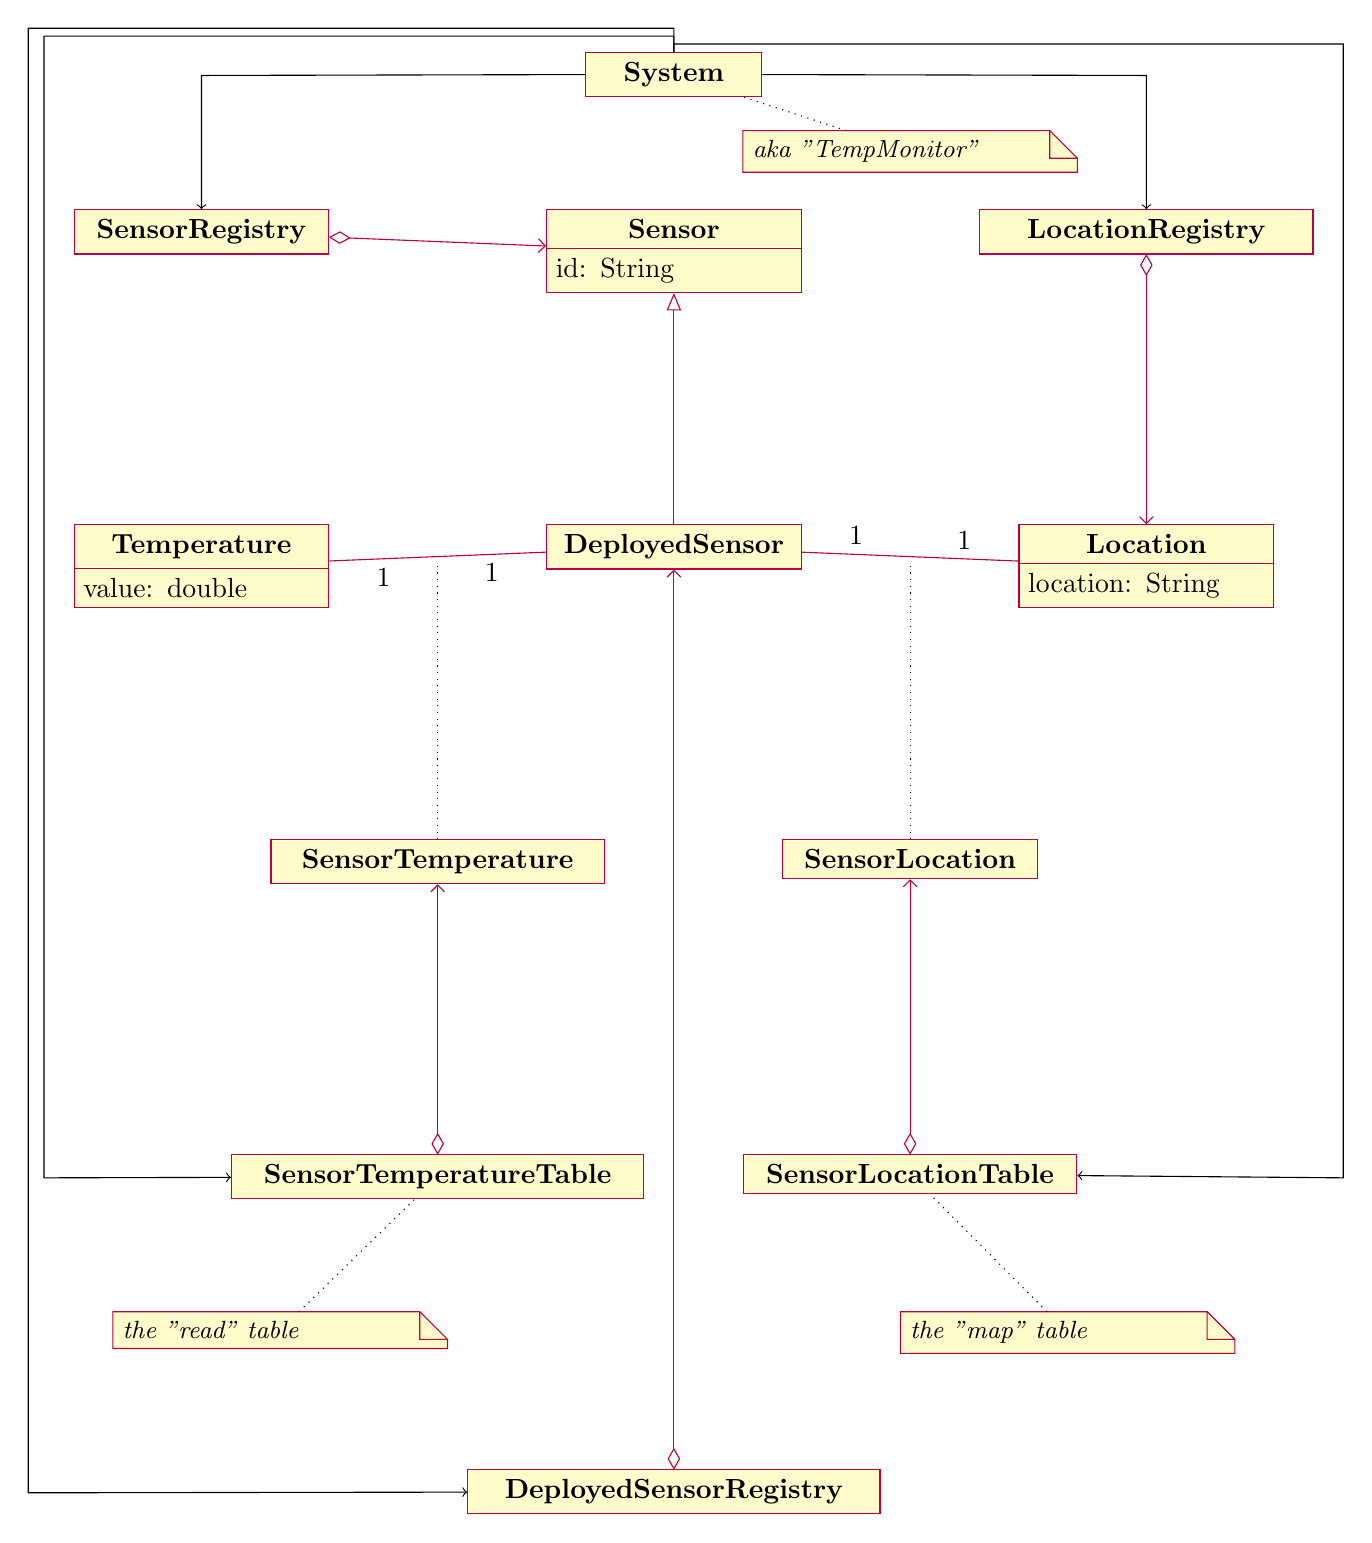
\begin{tikzpicture}

        % Defining the classes and their attributes
        \begin{class}[text width=2cm]{System}{0,6}
        \end{class}
        
        \begin{class}[text width=3cm]{SensorRegistry}{-6,4}
        \end{class}
        
        \begin{class}[text width=3cm]{Sensor}{0,4}
            \attribute{id: String}
        \end{class}
        
        \begin{class}[text width=4cm]{LocationRegistry}{6,4}
        \end{class}

        \begin{class}[text width=3cm]{Location}{6,0}
            \attribute{location: String}
        \end{class}
        
        \begin{class}[text width=3cm]{DeployedSensor}{0,0}
            \inherit{Sensor}
        \end{class}

        \begin{class}[text width=3cm]{Temperature}{-6,0}
            \attribute{value: double}
        \end{class}

        \begin{class}[text width=4cm]{SensorTemperature}{-3,-4}
        \end{class}

        \begin{class}[text width=3cm]{SensorLocation}{3,-4}
        \end{class}

        \begin{class}[text width=5cm]{SensorTemperatureTable}{-3,-8}
        \end{class}

        \begin{class}[text width=4cm]{SensorLocationTable}{3,-8}
        \end{class}

        \begin{class}[text width=5cm]{DeployedSensorRegistry}{0,-12}
        \end{class}

        % Defining the links between the classes
        \association {DeployedSensor}{1}{}{Location}{1}{}
        \association {DeployedSensor}{1}{}{Temperature}{1}{}
        \aggregation{SensorRegistry}{}{}{Sensor}
        \aggregation{DeployedSensorRegistry}{}{}{DeployedSensor}
        \aggregation{LocationRegistry}{}{}{Location}
        \aggregation{SensorLocationTable}{}{}{SensorLocation}
        \aggregation{SensorTemperatureTable}{}{}{SensorTemperature}

        % Manual associations
        \draw[->] (System) -- (-6, 5.7) -- (SensorRegistry);
        \draw[->] (System) -- (6, 5.7) -- (LocationRegistry);
        \draw[->] (System) -- (0, 6.1) -- (8.5, 6.1) -- (8.5, -8.3) -- (SensorLocationTable);
        \draw[->] (System) -- (0, 6.2) -- (-8, 6.2) -- (-8, -8.3) -- (SensorTemperatureTable);
        \draw[->] (System) -- (0, 6.3) -- (-8.2, 6.3) -- (-8.2, -12.3) -- (DeployedSensorRegistry);
        \draw[dotted] (SensorTemperature) -- (-3, -0.5);
        \draw[dotted] (SensorLocation) -- (3, -0.5);

        % Notes
        \umlnote(note1) at (3,5){\textit{\small aka "TempMonitor"}};
        \draw[dotted] (note1) -- (System);
        \umlnote(note2) at (-5,-10){\textit{\small the "read" table}};
        \draw[dotted] (note2) -- (SensorTemperatureTable);
        \umlnote(note3) at (5,-10){\textit{\small the "map" table}};
        \draw[dotted] (note3) -- (SensorLocationTable);
    
    \end{tikzpicture}
\end{document}
